\chapter{Theoretical background}

\label{ch:theoretical}
In the next part of the paper we will talk a bit more about the technologies and the concepts used in the making process, in order to offer a better understanding of the project. We'll start by presenting the building parts of Gitfs, from file system to git internals, and end up also discussing about similar projects. 

\section{File systems}
    A file system is an abstraction used by the operating systems in order to keep track of files on a storage device. In a more concrete form, you can see the file systems as a collection of data structures and algorithms which helps the operating system to manage data from a storage device. The operating system provides an API, which other programs can use to store, retrieve or delete data, from a storage device.
    
    The operation of associating a file system to a storage device is called `mounting`. In UNIX based operating systems, you can use the 'mount' command, which will attach a file system to the current file system hierarchy. Using the 'mount' command, you can specify a file system, its type, specific options used by the file system and a mounting point.

    \subsection{High level architecture}
        The actual structure of a file system can vary based on the implementation, but the majority of UNIX file systems, share a common one. It is composed by two main parts: user space and kernel space. 
        
        User space contains the applications (for this example, the user of the file system) and the GNU C Library (glibc), which provides the user interface for the file system calls (open, read, write, close). The system call interface acts as a switch, funneling system calls from user space to the appropriate endpoints in kernel space. 
        
        \begin{figure}[h]
           \begin{center}
               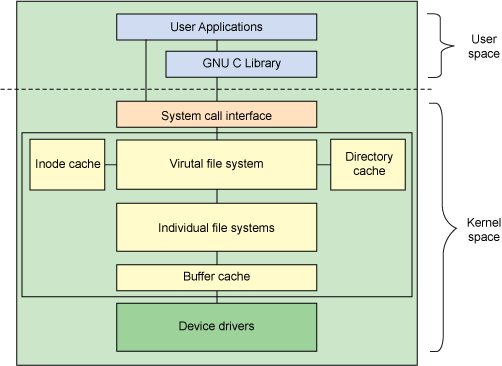
\includegraphics[width=15cm]{theoretical/filesystem-arhitecture.png}
            \end{center}
        \end{figure}

        As you can see in this figure, an important part of a file system architecture stays in the kernel space. There, the Virtual File System (VFS) behaves as an interface for other file systems. It behaves like a gateway between system call interface and individual file systems, with some caches. It does that by exposing a series of interfaces to individual file systems, optimizing using two caches: dentries (directory cache) and inode. Each one of those caches stores the recently-used objects (implementing a LRU cache mechanism).
        
        A kernel space implemented file system won't interact with a device directly. All write and read operations are passed through a cache, called a buffer cache. This is a very smart mechanism that offers a big performance boost, but with a cost. If you use the system call interface in order to write something in a file, that write is not atomic, meaning that if you close the file, the bits that you are writing are not on the storage device, but in this buffer cache. The kernel will flush periodically this cache on the device, but also can control the flushing using fsync system call, after you close the file. The buffer cache will use a LRU (Least Recently Used) cache which means that is a finite small cache that will store the most recent data, being optimized for use cases when you use the same data. 
        
        Linux uses multiple types of data structure to manage the entire file system:
        \begin{itemize}
            \item superblock: the root of file system, which maintains and describes state in the file system. It contains all the information needed by the file system during certain operations, such as: file system name (e.g.: ext2, ntfs, fat32 etc.), the size of the file system and its state, a reference to a block device and metadata. It is usually stored on the storage device but it can also be created at runtime. Besides that information, a superblock also contains a set of operations. This structure is used in order to manage the inodes within the file system.
            \item inode: core representation in a file system. Every file or directory is represented as an inode.
            It contains all the meta data needed by the file systems (including which operations are possible on it) to manage a file. Individual file systems will provide different functions and mechanisms in order to generate a unique inode identifier from a filename and later into an inode reference.
            \item dentry: data structure used to map the names of files to inodes. It uses a directory cache to keep the most-recently used data closely. The operating system also uses dentries to travers the file system.
            \item file: or VHS file is just an open file. It keeps the state for a given open file, such at write offset.
        \end{itemize}

        In order to dynamically add or remove a file system from Linux, a set of registration functions needs to be used. You can view a list of supported file systems, accessing the /proc file system, from user space. It's not a file on disk, but a virtual file from which you can find out which devices are currently associated with the file systems. If you want to add a new file system to Linux, you need to call register\_file system. The function takes only one argument which defines the reference to a file system (file\_system\_type) using the name of the file system, two superblock functions and a set of attributes. Once a file system is registered it can also be unregistered.

    \subsection{User space}
        Besides programming an individual file system in the kernel space you can use FUSE. FUSE stands for file system in user space and it is an interface for programs which helps you export a file system to the Linux kernel. It has two main components: libfuse and fuse kernel module. Libfuse is a C library which allows you to communicate with the FUSE kernel module.
        
        After the FUSE file system is mounted, all system calls which target that mountpoint will be redirected to the FUSE kernel module, acting like a proxy.
        
        \begin{figure}[h]
           \begin{center}
               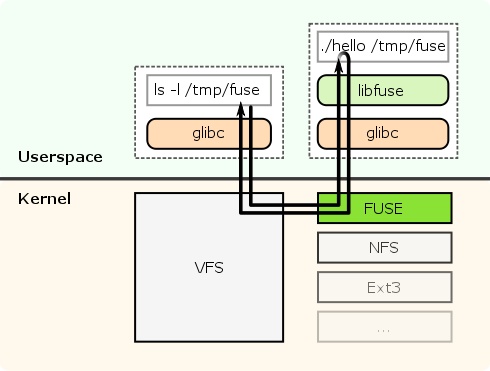
\includegraphics[width=15cm]{theoretical/fuse.png}
            \end{center}
        \end{figure}
         
        Let's take read operation as an example. Let's imagine that the directory /fuse is the FUSE mountpoint. When an application will call the read() syscall with /fuse/file as the path argument, the Virtual File System will trigger the corresponding handler in fusefs. A cache is used in order to optimize the operations flow. If the corresponding data is found in the cache it will be returned. Otherwise, the read() syscall will be forwarded to the libfuse library, which will call the callback defined in userfs for the read() syscall. The callback can make any action and return any data in the supplied buffer. With this mechanism one can implement any desired logic. For example, you can access Facebook's API in order to retrieve some photos, or to get data from an external storage device, or to do some processing from a local file system. After you've finished your work, the result is propagated to libfuse, through kernel and to the actual application which triggered the read() syscall. All file system operations can be implemented in the same manner.
        
        In order to allow non privileged users to mount the file systems, the fusermount utility was created. It also offers the possibility to customize several parameters when one mounts a file system.
        
        FUSE exposes two different APIs used to develop the file system:
        \begin{itemize}
            \item low-level: using this API the file system will need to manage the inodes and path translations (also caching for the translations), copying the VFS interface very closely. Also, the file system will need to manually fill and use the data structures used to communicate with the kernel. This API is mostly used to develop file system from scratch (take a look at ZFS-FUSE), in contrast to those that are just adding some functionality to existing file systems (extending them). 
            \item high-level: opposing the low-level API, using this level will force the file system developer to deal only with pathnames, not inodes and dentries, copying more the system calls interfaces than Virtual File System interface. Also, there is no need for any caching mechanism for inode-to-pathname translations and the data structures used for kernel communication are already filled. This API is used by the vast majority of FUSE-based file systems, taking care of most of the work in order to let the file system developer build the desired logic.
        \end{itemize}
        
        The vast majority of FUSE-based file systems are implemented as standalone applications that link with libfuse and use the high-level API to implement a specific behaviour. Because of the FUSE (kernel module) acts like a proxy to a libfuse based application, the performance is drastically lower than a usual kernel file system. Even though the performance may be lower, the speed of development is drastically improved. Libfuse has bindings in all major high level languages. Also, because FUSE will take care of inodes, dentries and caching the inode-to-pathname translations, the margin for errors is drastically reduced.
        
\section{Git}
    Git is one of the most popular distributed version control systems and it is also free and open source. It was originally created by Linus Torvalds with the purpose of improving Linux development which had become very cumbersome to maintain, due to the large number of patches that needed to be reviewed and integrated in the kernel.
    
    The central component of git is the repository. A repository is a directory which contains all the necessary files that git uses to manage the content and the history. This repository can be bare, containing only the necessary parts without the content itself, or non-bare and including the content.
    
    In order to get a repository on the local system you need to clone it. You can clone a repository from a local machine or a remote one. Git can use different protocols in order to clone a repository (ssh, http/https or git protocol). Every change that was managed by git can be pushed to a remote repository. Each repository, on which you want to push or from which you want to pull changes, has an address and a name. The data structure that encapsulates these attributes is called a remote. You can have multiple remotes on a local repository, with different addresses but with unique local names. The default remote (initially used to clone the repository) is called origin.
    
    Using remotes you can distribute the code and work offline. Changes can be synchronized between multiple remotes and any raising conflicts would be solved automatically (if possible).
    
    \subsection{Overview}
        After a remote repository is cloned on the local machine, one can start changing its content. Git will track only the files that are already in the repository. Newly created files need to be manually added as tracked. Empty directories are not track-able.
        
        Any new changes are viewed and tracked by git, but not automatically transformed in a version. In order to group the changes, git uses the concept of stage. Each new change is tracked by git in the so called working stage. In this zone, the changes are very volatile. If you want to pull content from a different remote, git will stop you in order to save the local changes. In order to group them, you need to add the changed files to the staging area, by using `git add` command.
        
        Once you group the changes together, by moving the files to the stage area, you can create a version. That version is named commit. A commit is a git object, which contains a group of files that were changed, the name of who made the changes, who created the commit and the time of when these happened. Besides this metadata, git will attach an unique hash to it in order to be easily identifiable and a reference to the previous commit, called parent. In this way, git can offer an ordered log (not by time, but the order of changes, because you can rewrite the history and relocate a given commit in its tree of changes) giving you a broader understanding of the changes that were made.
        
        Given the fact that each commit has a parent, you can easily form a chain of commits, called a branch. You can create as many branches as you want, starting with a commit. The default branch is considered to be the master. A branch can be created just locally and pushed to any remote repository afterwards. The last commit from a given branch is called HEAD.
        You can change the HEAD at any time, changing the state of the local or remote repository.
        
        \begin{figure}[h]
           \begin{center}
               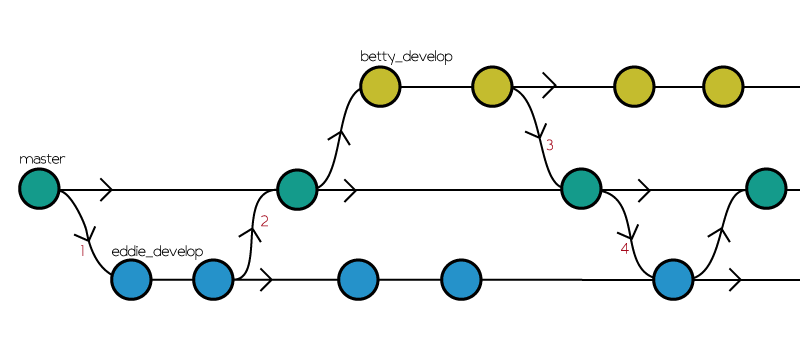
\includegraphics[width=15cm, height=8cm]{theoretical/git_flow.png}
            \end{center}
            \label{fig:git-flow}
            \caption{Git's chain of commits}
        \end{figure}
        
        From a commit two branches can diverge, as showed in figure ~\ref{fig:git-flow}. If you want to bring commits from another branch to a given current branch, you can do that by using one of two methods: rebasing or merging. 
        Using the rebase method you will apply the current commits (set of changes) to the last commit of the branch you want to rebase into, in the order of which the commits were created, one by one. Any conflicts will be solved at commit level, if this will be the case. 
        The merging method will try to apply the changes without keeping track of the order of the commits. All conflicts will be solved at the end of the operation and will end with a commit. 
        The safest and cleanest method is the rebase method, but a big inconvenience is that it will rewrite the history, creating new commits (with the same data and metadata: date, author, commiter etc.) for each commit applied.
        
        You can use any of these methods in order to apply remote changes to current state of the content. Git can manage the branches from all the remotes and using some porcelain commands, you can decide which changes to be applied to the local content.
        
        Another useful structure offered by git is the tag. A tag is a frozen reference which will point to given state in the repository, just like a commit. Unlike a commit, a tag can't be changed and has no parent. Tags are used in order to froze the state of a given repository. 
        
        You can imagine the entire repository like a tree, with multiple branches. The local repository will point to a certain reference. This reference can be a tag, the head of a branch or just the hash of a commit. In this way, you can easily change the state of your repository, by checking-out on different references. The checkout operation can have multiple modes (soft, hard) and in case of conflicts, you can solve them manually or by accepting the local changes (referred as ours) or the remote ones (referred as theirs).
        
    \subsection{Internals}
        Until now we have talked about git more from a functional point of view, like a tool. But git can be viewed like a database as well or, more precisely, like a key-value database. In this way, one can refer to git as a content addressable file system. You can add any type of content into it and receive a key which you can use to retrieve the content back. In order to investigate this further we need to take a look at dot git directory.
        
        Dot git directory contains all the data and the meta data of our repository. The part of meta data is stored in the very descriptive files. Some of the most important are:
        
        \begin{itemize}
            \item HEAD: the current reference to which your repository points. Usually it will be refs/heads/master
            \item refs: all known references, grouped by remotes. Here you will also find the mapping between branches and commits.
            \item index: the staging area with it's meta data, like file names, timestamps and hashes of the files managed by git.
        \end{itemize}
        
        Beside those meta data files, dot git directory hides the entire repository's state and history in a directory called objects. Git will store every file ever changed in two type of data structures: tree and blob. Each such object is represented by an unique hash. SHA-1 hash function is used, over the content and the meta data of an object, in order to generate a hash. That hash is used to map an object to it's content. The content is archived (using the zip format) and stored on the disk, in objects directory using the hash as name for the file.
        
        It's very similar to how an UNIX file system manages the files. The tree objects will correspond to an UNIX directory and a blob to, more or less, an inode or file contents. Every tree object can contain one or more trees, each of them contains a SHA-1 pointer to a blob or a subtree, having associated file name, mode and type. Git will create those objects by retrieving the state of your repository (staging area and index) and writing tree objects from them. It will create new objects only for changed files and reuse old nodes if their corresponding files were not changed. In this way git can optimize disk memory usage.
        
        As git will not store empty directories, the leafs will be all the time blobs, not trees.
        
        \begin{figure}[h]
           \begin{center}
               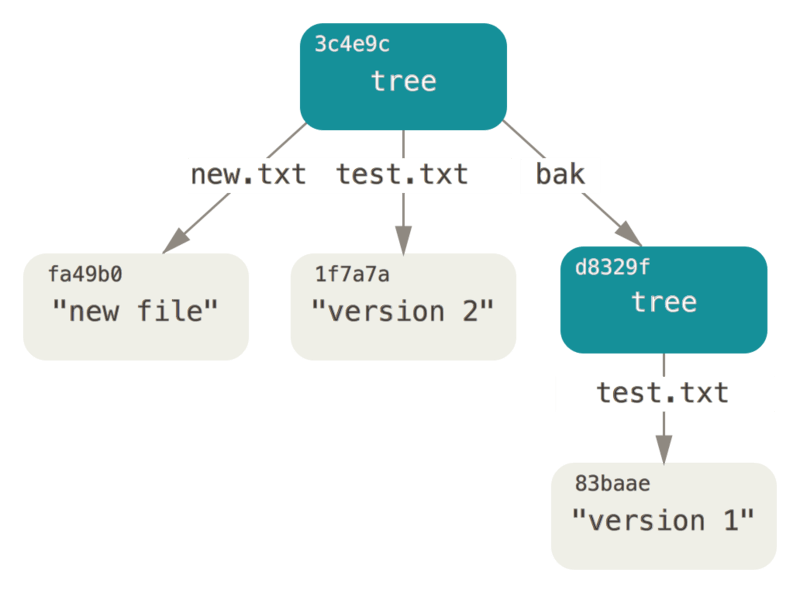
\includegraphics[width=15cm]{theoretical/data-model-2.png}
            \end{center}
            \label{fig:git-objects}\caption{Git data model}
        \end{figure}
        
        As one can observe, by using this mechanism a tree is formed for the current state of the repository (and it will be used to compose other version of the repository). This tree data structure is based on Merkle tree, a type of tree in which all the nodes are uniquely identified by a hash, except the leafs. This data structure is very efficient for lookup operations, which can be done in O(logn) time. In this kind of tree, if a node's hash is changed, all the nodes up to the root need to update their hashes. In this way, git will create a new tree for each commit you create, but in that tree, the nodes that were not changed, will be reused.
        
        Another important object is the commit object. This object will store a reference (SHA-1 hash) to the root of a the current tree (which represents a snapshot of the current state of the repository), a reference to the previous commit (called parent), the author and commiter (can be separate persons) and a blank line followed by the commit message. In this manner, a graph will be formed.
        
         \begin{figure}[h]
           \begin{center}
               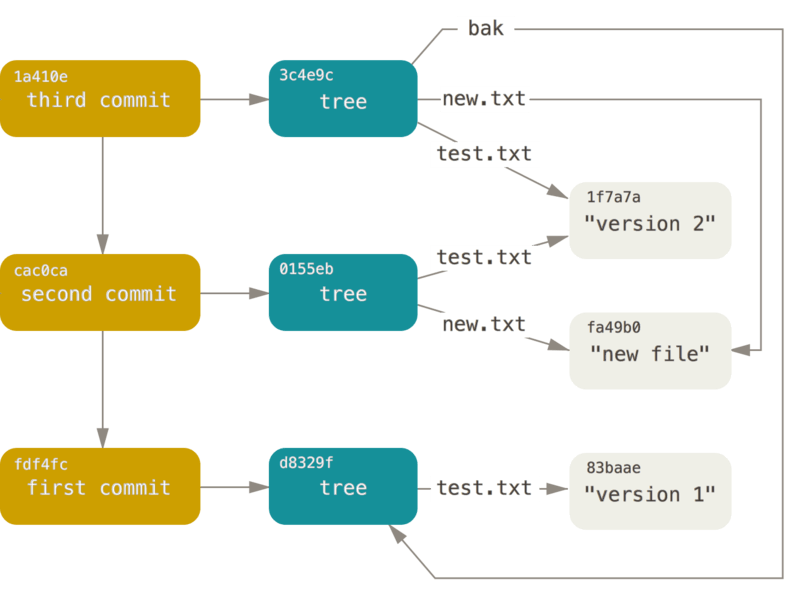
\includegraphics[width=15cm]{theoretical/data-model-3.png}
            \end{center}
            \label{fig:git-objects}\caption{Git's objects and their relations}
        \end{figure}
    
\section{Python}
    Python is a popular, general-purpose, high-level programming language. It was designed with a strong accent on code readability and an easy to learn syntax which makes it a very easy language to learn and maintain. The language has a lot of constructs intended to create clear and readable small and large scale programs. Using those constructs programmers can express complex ideas much faster, cleaner and in fewer lines of code, compared to other high-level languages as Java, C\# or C++. It's ancestor, abc language, was created with the purpose to be a teaching language and Python inherited a large part of it.
    
    One of its first usages (remaining today as an important and large one) was as a scripting language, used for servers administration. Being a high-level programing language it also supports different programming paradigms: object-oriented, functional, imperative or procedural. As a scripting language, it has a dynamic type system and automatic memory management with a large standard library.
    
    Starting first as a scripting language used for server administration, a lot of system programming features emerged, making it a strong candidate for file systems development.
    
    Python is the specification of a language. Its implementation varies, depending on which subset one wants to implement and in what language. The reference implementation in C language is called CPython. It is the most popular one and it is found already installed in almost any Linux distribution. PSF (Python Software Foundation, non-profit) manages all CPython development.
    
    \subsection{Advantages}
        \begin{enumerate}
           \item Python is dynamically typed: it means that you don't declare a type (e.g. 'integer') for a variable name, and then assign something of that type (and only that type). Instead, you have variable names, and you bind them to entities whose type stays with the entity itself. a = 5 makes the variable name a to refer to the integer 5. Later, a = "hello" makes the variable name a to refer to a string containing "hello". Statically typed languages would have you declare int a and then a = 5, but assigning a = "hello" would have been a compile time error. On one hand, this makes everything more unpredictable (you don't know what a refers to). On the other hand, it makes it very easy to achieve results which static typed languages make very difficult.
           \item Python is strongly typed. It means that if a = "5" (the string whose value is '5') will remain a string, and never coerced to a number if the context requires so. Every type conversion in python must be done explicitly. This is different from Perl or Javascript,for example, where you have weak typing and can write things like "hello" + 5 to get "hello5".
           \item Python is object oriented, with class-based inheritance. Everything is an object (including classes, functions, modules, etc), in the sense that they can be passed around as arguments, have methods and attributes, and so on.
           \item Python is multipurpose: it is not specialised to a specific target of users (like R for statistics, or PHP for web programming). It is extended through modules and libraries, that hook very easily into the C programming language.
           \item Python enforces correct indentation of the code by making the indentation part of the syntax. There are no control braces in Python. Blocks of code are identified by the level of indentation. Although a big turn off for many programmers not used to this, it is precious as it gives a very uniform style and results in code that is visually pleasant to read.
           \item The code is compiled into byte code and then executed in a virtual machine. This means that precompiled code is portable between platforms.
        \end{enumerate}
        
    \subsection{CFFI}
        There are various tools which make it easier to bridge the gap between Python and C. One of the most used and spread tool is CFFI (C Foreign Function Interface).
        
        FFI refers to the ability of code written in one language (the “host language,” such as Python), to access and invoke functions written in another language (the “guest language,” such as C). The term “foreign” refers to the fact that the functions come from another language and environment.
        Depending on the language and its FFI support, you might also be able to access global named variables, automatically convert data types between the host and guest languages, and have code in the guest language invoke functions in the host language as callbacks.
        
        In interpreted languages like python, it’s usually not possible to use a library’s compile-time features like C preprocessor macros and constants (i.e. things \#define’d in the library headers). This is because the FFI accesses the library’s binary code (e.g. its .so, .dylib, or .dll) directly, without compiling any code.
        However, the FFI support in some compiled languages works by compiling down to C code; in these cases, you may be able to use compile-time features. It all depends on the language and how it implements FFI.
        
        CFFI can be used in one of four modes: “ABI” versus “API” level, each with “in-line” or “out-of-line” preparation (or compilation).The ABI mode accesses libraries at the binary level, whereas the API mode accesses them with a C compiler.
        In the in-line mode, everything is set up every time you import your Python code. In the out-of-line mode, you have a separate step of preparation (and possibly C compilation) that produces a module which your main program can then import.
    \subsection{Fusepy}
        Fusepy is a Python module that provides a simple interface for FUSE and MacFUSE. It is just one file and it is implemented using ctypes.

        The original version of fusepy was hosted on Google Code, but is now officially hosted on GitHub.
       
        Fusepy is written in 2x syntax, but it is trying to also pay attention to bytes and other changes 3x would care about. The only incompatible changes between 2x and 3x are the changes in syntax for number literals and exceptions.
    \subsection{Libgit2}
        Libgit2 is a library written in C which manipulates the git objects at as low level as possible. It follows git implementation and offers an API which helps developers in creating applications that use git, without the use of the git binary.
        
        A great advantage of Libgit2 is that it is written in C, offering bindings in all major high level languages, using CFFI (C Foreign Function Interface). It offers features like, cloning a repository, creating commits, merging commits and fetching changes from different remote repositories.
        
    \subsection{Pygit2}
        One of the languages in which Libgit2 has bindings is Python. The implementation of Libgit2 in Python is called Pygit2. It uses CFFI and Python C Objects in order to bring the functionalists of Libgit2 into Python world.
        
        It is a portable library, having releases for Linux, Windows and MacOS, with a small community, but plenty of contributions.
        
        Because Python is an object oriented programming language, Pygit2 exposes all of Libgit2's data structures as classes. In this way, Pygit2 offers a mechanism which allows you to extend the functionalists from Libgit2. From those data types, the Repository is the one which encapsulates the most of part the behaviour, using other data types like Remote, Branch and Commit.
    
\section{Similar Projects}
    \subsection{ZFS}
        ZFS is a combined file system and logical volume manager designed by Sun Microsystems. The features of ZFS include protection against data corruption, support for high storage capacities, efficient data compression, integration of the concepts of file system and volume management, snapshots and copy-on-write clones, continuous integrity checking and automatic repair.
        
        ZFS uses a copy-on-write transactional object model. All block pointers within the file system contain a 256-bit checksum or 256-bit hash (currently a choice between Fletcher-2, Fletcher-4, or SHA-256) of the target block, which is verified when the block is read. Blocks containing active data are never overwritten in place; instead, a new block is allocated, modified data is written to it, then any metadata blocks referencing it are similarly read, reallocated, and written. To reduce the overhead of this process, multiple updates are grouped into transaction groups, and ZIL (intent log) write cache is used when synchronous write semantics are required. The blocks are arranged in a tree, as are their checksums (see Merkle signature scheme).
        
        An advantage of copy-on-write is that, when ZFS writes new data, the blocks containing the old data can be retained, allowing a snapshot version of the file system to be maintained. ZFS snapshots are created very quickly, since all the data composing the snapshot is already stored. They are also space efficient, since any unchanged data is shared among the file system and its snapshots.

        Writeable snapshots ("clones") can also be created, resulting in two independent file systems that share a set of blocks. As changes are made to any of the clone file systems, new data blocks are created to reflect those changes, but any unchanged blocks continue to be shared, no matter how many clones exist. This is an implementation of the Copy-on-write principle.
        
    \subsection{SparkleShare}
        SparkleShare is an open source software which offers you the possibility to share a directory with more collaborators and create versioned content. It is presented as a standalone application in which an user can setup multiple projects (different directories) which will get synchronized with other collaborators' changes.
        
        It uses git as storage layer, which gives you the possibility to control where your data is stored, in order to protect your privacy. To make setup easier, the team which developed SparkleShare also developed a series of scripts which automate private git host creation. Beside those scripts, you can use any git hosting services, from Github, Bitbucket (which are proprietary solutions) to Gitlab or Gogs (open source solutions).
        In order to help you maintain the privacy it also includes client side encryption.
        
        It is written in C\# and it uses git command line tool for git operations. Being written in C\# it has some drawback for portability, but it can compensate with higher code maintainability and extensibility options, and also performance boost. Unfortunately, the performance boost given by C\#, will be annulled by the overhead in using the git command line tool. Spawning processes for each git command can lead to complicate error handling logic and resource heavy usage, because you rely on the git's command line tool implementation.
        
        Beside file synchronization, it also offers the possibility to revert files. It is suitable for small files (from text to media files), but that great when it come to large binary files, full computer backups or large collection of files. 